%% Makros for Kompendium


%% Text nur bei deutscher Sprache ausgeben:
\NewDocumentCommand{\deu}{m}{%
\ifthenelse{\equal{\kLanguage}{deu}}{%%
{#1}}{%%
}%% end ifthenelse
}% end deu

%% Text nur bei englischer Sprache ausgeben:
\NewDocumentCommand{\eng}{m}{%
\ifthenelse{\equal{\kLanguage}{eng}}{%%
{#1}}{%%
}%% end ifthenelse
}% end eng


%%%%%%%%%%%%%%%%%%%%%%%%%%%%%%%%%%%%%%%%%%%%%%%%%%%%%%%%%%%5
\newcounter{aufgabenNummer}
\setcounter{aufgabenNummer}{1}


\NewDocumentCommand{\isLoesungen}{m}{%%
\ifthenelse{\equal{\kLoesungen}{true}}{%%
#1}{%%
}%% end ifthenelse
}%%

\NewDocumentCommand{\isAufgaben}{m}{%%
\ifthenelse{\equal{\kLoesungen}{false}}{%%
#1}{%%
}%% end ifthenelse
}%% end IS Aufgaben


\newcommand{\mmPapierZwei}[2]{\begin{tikzpicture}
%%  \draw[step=4mm,bbwMMFarbe,ultra thin]
%%  \draw[step=4mm,bbwMMFarbe,thick]
  \draw[step=5mm,gray,line width=0.02mm]
  (0, 0) grid ({#2}, {#1});
\end{tikzpicture}}%%



\NewDocumentCommand{\isMMPapier}{m}{%%
  \ifthenelse{\equal{\kMMPapier}{true}}{%%
    
    \mmPapierZwei{#1}{17.0}

}{%%
}%% end ifthenelse
}%%

\newcommand{\nurNiveauBMP}[1]{%%
\ifthenelse{\equal{\kAufgabenNiveau}{bmp}}{%%
#1
}%% end ifthenelse
}%%

\newcommand{\auchTrainingsAufgabe}[1]{%%
\ifthenelse{\equal{\kAufgabenNiveau}{bmp}}{%%
%% Aufgabennummern durchnummerieren, auch wenn keine Trainingsaufgaben
%% ausdedruckt werden
\stepcounter{aufgabenNummer}%%
}{%%
#1
}%% end ifthenelse
}%%

\newcommand{\fragenMarkierung}{}

%% Kompendium Aufgaben
%% #1 : Aufgabentext
%% #2 : Lösungstext
%% #3 : Optional, 

%% Jedes Kapitel beginnt mit neuen Buchstaben.
%% Algebra hat Aufgabne A1, A2. ,,, Funktionen F1, F2, ...
%%
\newcommand{\kAufgabenBuchstabe}{0}
\newcommand{\kMetaAufgabe}[3]{%%
  \kAufgabenBuchstabe{}\,\arabic{aufgabenNummer}. \fragenMarkierung{}:
  \isLoesungen{{\color{blue}#2}}\isAufgaben{#1}\stepcounter{aufgabenNummer}
  \isMMPapier{#3}
  \vspace{2mm}
}%% end kaufgabe

\newcommand{\kNiveauAufgabe}[3]{%%
%%\nurNiveauBMP{\kMetaAufgabe{#1}{#2}{#3}}%%
\renewcommand{\fragenMarkierung}{\colorbox{red!30}{(B)}}
\kMetaAufgabe{#1}{#2}{#3}%%
}%% end kaufgabe

\newcommand{\kTrainingAufgabe}[3]{%%
\renewcommand{\fragenMarkierung}{\colorbox{blue!30}{(E)}}
\auchTrainingsAufgabe{\kMetaAufgabe{#1}{#2}{#3}}%%
}%% end kaufgabe


\renewcommand{\indexname}{\deu{Stichwortverzeichnis}\eng{Index}}%%

%% Layout erste Seite
\newcommand{\printKFirstPage}{%%
  \thispagestyle{empty}
  \begin{center} {\huge{Kompendium}} \end{center}

  \vspace{10mm}
  
  \begin{center} {\large{GESO}} \end{center}

  \begin{center}
    \isLoesungen{\deu{Lösungsteil}\eng{Solutions}}
    \isAufgaben{\deu{Aufgabenteil}\eng{translate: Excercises}}
  \end{center}

  \vspace{10mm}

  \begin{center} \deu{deutsche Version} \eng{english version} \end{center}
  \vspace{10mm}

\vspace{60mm}

\begin{center}\begin{small} \deu{Autoren} \eng{Authors}\\
Susanne Wagner (susanne.wagner@bms-zuerich.ch)\\
Thomas Fellmann (thomas.fellmann@bms-zuerich.ch)\\
Mirjam Bräm, Wolfgang Pfalzgraf, Ulrike Gruber
Urs Vonaesch\\
Christian Hersberger (christian.hersberger@bmwin.ch)\\
Phlipp Freimann (philipp.freimann@bmwin.ch) \end{small}
  \end{center}


  \vspace{20mm}

  \begin{center}Kantonale Ausgabe \kVersion{} Kanton Zürich \end{center}

  
\newpage

  \ifthenelse{\equal{\kAufgabenNiveau}{bmp}}{%% nothing
}{%%
 \deu{Mit {\colorbox{blue!30}{(E)}} gekennzeichnete Aufgaben dienen
lediglich dem Training als Einstiegsaufgaben.\\
Mit \colorbox{red!30}{(B)} gekennzeichnete Aufgaben haben das Niveau
  der BMP (Berufsmaturitätsprüfung).
}%% end deu

\eng{Questions having \colorbox{blue!30}{(E)} are only for
    training purpouse.\\
Questions marked with  \colorbox{red!30}{(B)} have the level BMP (Berufsmaturitätsprüfung).
}%% end printKFirstPage
}%% end if Unterscheidung BMP

\newpage
\tableofcontents{}
\newpage
\pagestyle{fancy}
}%% end firstPage


%% Philipp G Freimann Juli 2019 für die BBW
%% Phi BBW-Vorlage für Mathematische Dokumente (LaTeX)
%% 2019 - 07 - 11
%%%%%%%%%%%%%%%%%%%%%%%%%%% M a t h e   M a k r o s %%%%%%%%%%%%%%%%%%%%%%%%%%%%%5

\usetikzlibrary{arrows.meta}

%% Kleine Symbole über anderen. Z. B. "?" über einem
%% Gleichheitszeichen:
%% Use \ueberMini{=}{?} um ein kleines Fragezeichen über ein
%% Gleichheitsszeichen zu schreiben.
\newcommand{\ueberMini}[2]{ \mathrel{\stackrel{\makebox[0pt]{\mbox{\normalfont\tiny #2}}}{#1}} }

%% Gleichungssystem mit zwei Zeilen und vier Einträgen (je zwei links
%% bzw. rechts).
\def\gleichungZZ#1#2#3#4{%%
  $$\left|
  \begin{array}{rcl}
    {#1} &=& {#2}\\
    {#3} &=& {#4}
    \end{array}\right|$$}%%

\def\gleichungDD#1#2#3#4#5#6{%%
  $$\left|
  \begin{array}{rcl}
    {#1} &=& {#2}\\
    {#3} &=& {#4}\\
    {#5} &=& {#6}\\
    \end{array}\right|$$}%%

%% Entspricht-Symbol
%%\usepackage{accents}
\newcommand{\hatset}[1]{\accentset{\wedge}{#1}}
\newcommand{\entspricht}{\,\,\hatset{=}\,\,}
\newcommand*\mittelwert[1]{\bar{#1}}
\newcommand*\mediantilde[1]{\widetilde{#1}}

%%
%% Graphiken mit tikz: BBW-Mathe-akros
%%
\tikzset{bbwgrid/.style={help lines,color=cyan!18, step=0.5cm}}

\newcommand{\bbwGridPart}[4]{
 % grid:
 \draw[bbwgrid] (#1,#3) grid (#2,#4);

 % axes
 \draw[thick] (#1,0) -- (#2,0);
 \draw[thick] (0,#3) -- (0,#4);
 \foreach \x in {#1, ..., -1}  \draw (\x cm, 2pt) -- (\x cm, -2pt)  node[anchor=north]{$\x$};
 \foreach \x in {1, ..., #2}   \draw (\x cm, 2pt) -- (\x cm, -2pt)  node[anchor=north]{$\x$};
 \foreach \y in {#3, ..., -1}  \draw (-2pt, \y cm) -- (2pt, \y cm)  node[anchor=east]{$\y\,\,$};
 \foreach \y in {1, ..., #4}   \draw (-2pt, \y cm) -- (2pt, \y cm)  node[anchor=east]{$\y\,\,$};
 \draw[->,thick] (#2,0) -- ({#2+0.5},0) node[anchor=west]{$x$};
 \draw[->,thick] (0,#4) -- (0,{#4+0.5}) node[anchor=south]{$y$};
}


%% A function within a Grid (without painting the grid)
%% #1: funciton eg 2*\x  (x has to be backquoted)
%% #2: Domain eg. -1:2.5
%% #3: colour eg red
\newcommand{\bbwFuncC}[3]{\draw[domain=#2,smooth,samples=200,variable=\x,#3] plot ({\x},{#1});
}
%% A function within a Grid (without painting the grid)
\newcommand{\bbwFunc}[2]{\bbwFuncC{#1}{#2}{blue}}

%% Declare a function-plot
%% xmin,xmax,ymin,ymax,fct,domain(x-min, x-max)
%% example: \bbwFunction{-4}{3}{-2}{5}{-\x*\x- \x + 4.5}{-3:2}
\newcommand{\bbwFunction}[6]{\begin{tikzpicture}
\bbwGridPart{#1}{#2}{#3}{#4}
 \bbwFunc{#5}{#6}
%% \draw[domain=#6,smooth,samples=200,variable=\x,blue] plot ({\x},{#5});
\end{tikzpicture}}
%% a whole graph having a coordinate-system #1-#4 and any tizpicture content #5:
\newcommand{\bbwGraph}[5]{\begin{tikzpicture}\bbwGridPart{#1}{#2}{#3}{#4}#5\end{tikzpicture}}

%% Dots and lines:
%% Dot example: \bbwDot{-1,2}{red}{east}{A}
\newcommand{\bbwDot}[4]{\filldraw[color=#2!60, fill=#2!5, thick](#1) circle(0.05) node[anchor=#3]{$#4$};}

%% Line example: \bbwLine{-1,0}{2,3}{red}
\newcommand{\bbwLine}[3]{\draw[thick,color=#3] (#1)--(#2);}

\newcommand{\bbwArrow}[3]{\draw[thick,color=#3,->] (#1)--(#2);}


%% Draw a single letter or small text
% #1: Position eg  4,4
% #2: letter eg f or blah
% #3: colour
\newcommand{\bbwLetter}[3]{\draw[color=#3](#1) node{$#2$};}

%%% ABC-Formel
%% usage \abcd{<a>}{<b>}{<c>}
%% example usage: \abcd{b}{5}{\sqrt{4}}
\newcommand{\abcd}[3]{$\frac{-(#2)\pm\sqrt{(#2)^2 - 4\cdot{}(#1)\cdot{}(#3)}}{2\cdot{}(#1)}$}



%% Trigonometrische Koordinatensysteme
%% Alle heißen "trigsysS" wobei da S einer der folgenden Sub-Systeme
%% bezeichnet:
%%  A  phi von  0 ... 360
%%     y   von -3 ...   3
%%
%%  B  phi von  0 ... 360
%%     y   von -1 ...   1
%%
%%  C  phi von  -270 ... 450
%%     y   von    -2 ...   2
%%
%%  D  phi von  -270 ... 450
%%     y   von    -1 ...   1
%%

\newcommand{\trigsysA}{
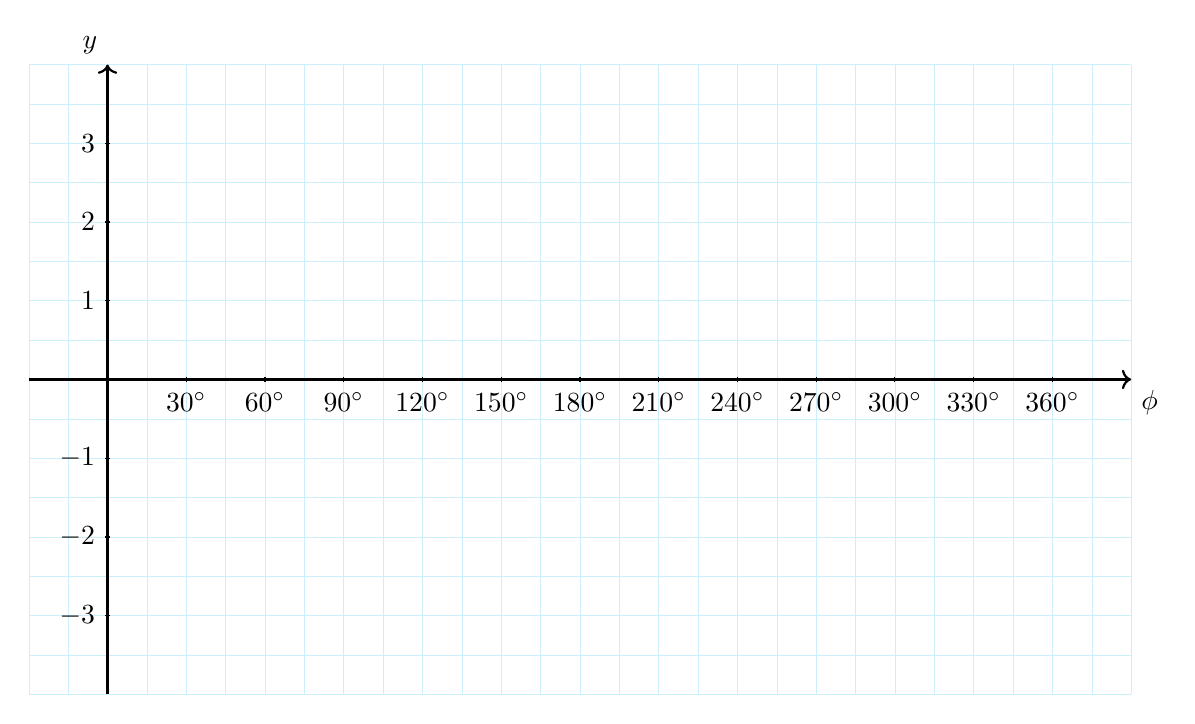
\begin{tikzpicture}
\draw[step = 0.5 cm, cyan!20 , very thin] (-1, -4) grid ( 13, 4);
\draw[thick, ->] (-1,0) -- (13,0) node[anchor = north west] {$\phi$};
\draw[thick, ->] (0,-4) -- (0,4) node[anchor = south east] {$y$};

\foreach \x [evaluate=\x as \degree using int(\x*30)] in {1,...,12}{ 
   \draw (\x cm, 1pt) -- (\x cm, -1pt) node[anchor = north] {$\degree^\circ$};
   }
\foreach \y in {-3,-2,-1,1,2,3}
   \draw (1pt, \y cm) -- (-1pt, \y cm) node[anchor = east] {$\y$};
\end{tikzpicture}}%% END Definition

\newcommand{\trigsysB}{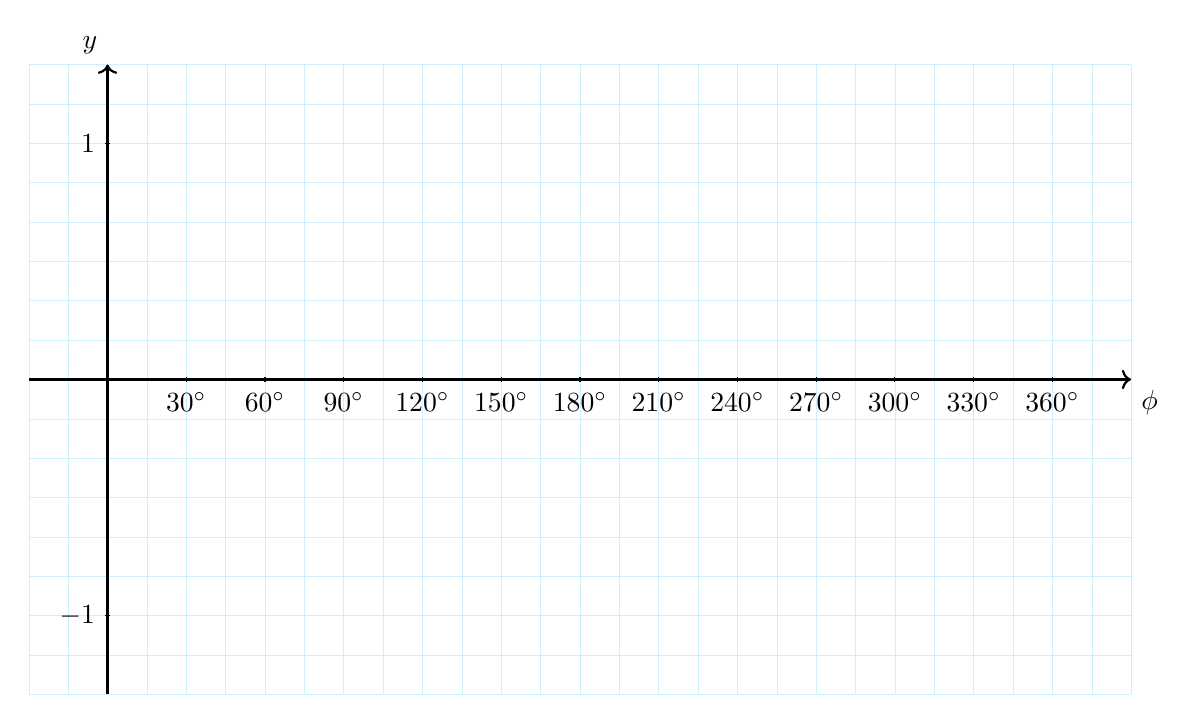
\begin{tikzpicture}\draw[step = 0.5 cm, cyan!20 , very thin] (-1, -4) grid ( 13, 4);
\draw[thick, ->] (-1,0) -- (13,0) node[anchor = north west] {$\phi$};
\draw[thick, ->] (0,-4) -- (0,4) node[anchor = south east] {$y$};

\foreach \x [evaluate=\x as \degree using int(\x*30)] in {1,...,12}{ 
   \draw (\x cm, 1pt) -- (\x cm, -1pt) node[anchor = north] {$\degree^\circ$};
   }
\foreach \y in {-1,1}
   \draw (1pt, \y *3cm) -- (-1pt, \y *3cm) node[anchor = east] {$\y$};

\end{tikzpicture}}%% END Definition

\newcommand{\trigsysC}{
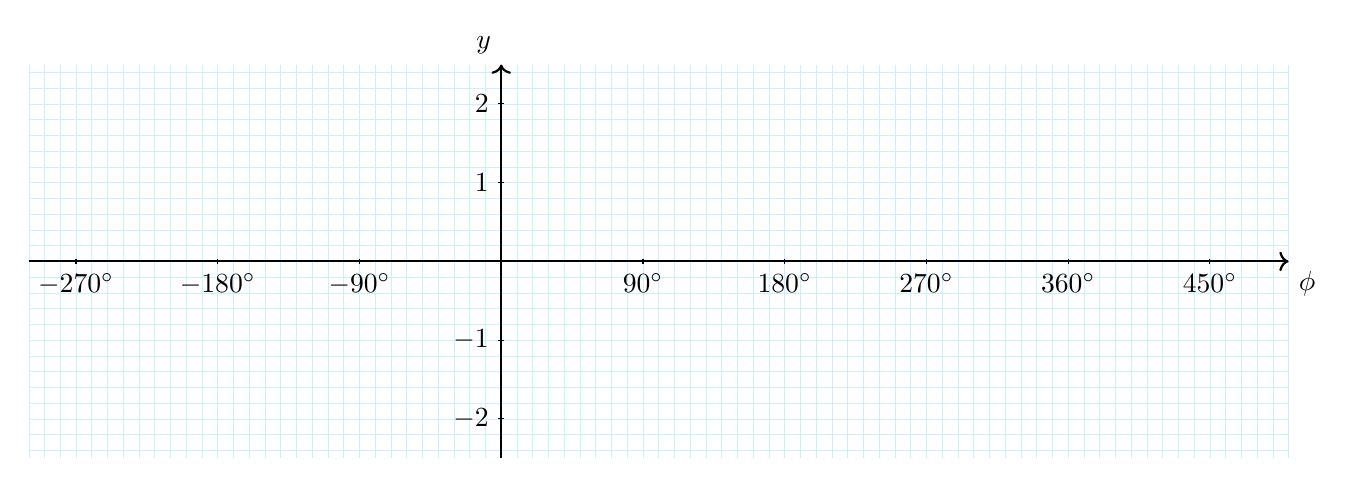
\begin{tikzpicture}
\draw[step = 0.2 cm, very thin, cyan!20] (-6, -2.5) grid ( 10, 2.5);
\draw[thick, ->] (-6,0) -- (10,0) node[anchor = north west] {$\phi$};
\draw[thick, ->] (0,-2.5) -- (0,2.5) node[anchor = south east] {$y$};

\foreach \x [evaluate=\x as \degree using int(\x*90)] in {-3,-2,-1,1,2,3,4,5}{ 
   \draw (\x *18mm, 1pt) -- (\x * 18mm, -1pt) node[anchor = north] {$\degree^\circ$};
   }
   
\foreach \y in {-2,-1,1,2}
   \draw (1pt, \y cm) -- (-1pt, \y cm) node[anchor = east] {$\y$};
\end{tikzpicture}}%% END Definition

\newcommand{\trigsysD}{
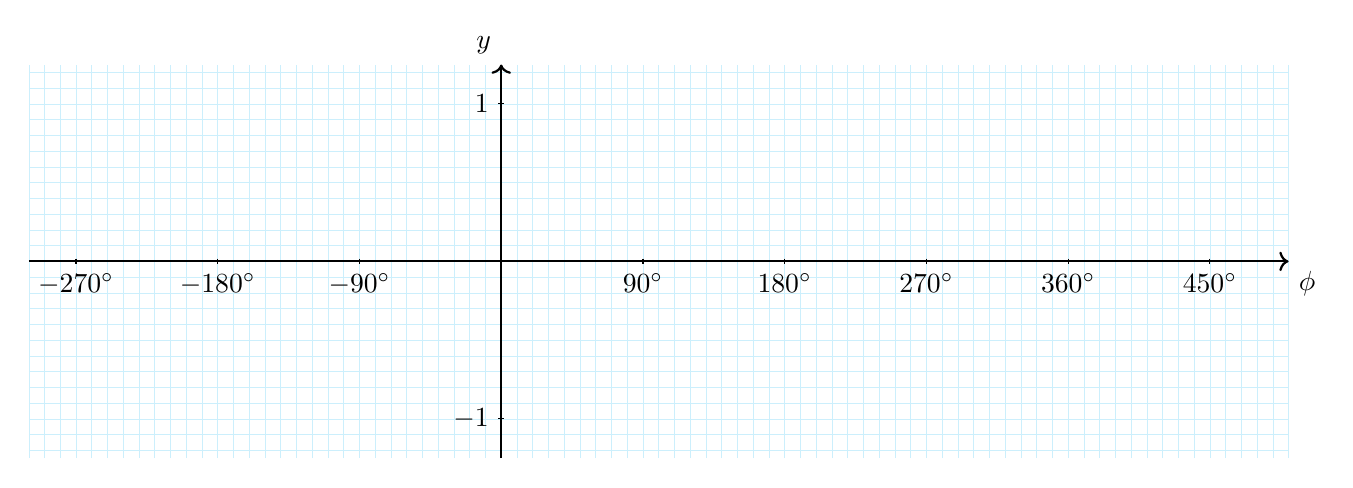
\begin{tikzpicture}
\draw[step = 0.2 cm, very thin, cyan!20] (-6, -2.5) grid ( 10, 2.5);
\draw[thick, ->] (-6,0) -- (10,0) node[anchor = north west] {$\phi$};
\draw[thick, ->] (0,-2.5) -- (0,2.5) node[anchor = south east] {$y$};

\foreach \x [evaluate=\x as \degree using int(\x*90)] in {-3,-2,-1,1,2,3,4,5}{ 
   \draw (\x *18mm, 1pt) -- (\x * 18mm, -1pt) node[anchor = north] {$\degree^\circ$};
   }
   
\foreach \y in {-1,1}
   \draw (1pt, \y *2cm) -- (-1pt, \y *2cm) node[anchor = east] {$\y$};
\end{tikzpicture}}%% END Definition


\newcommand{\trigsysDsin}{
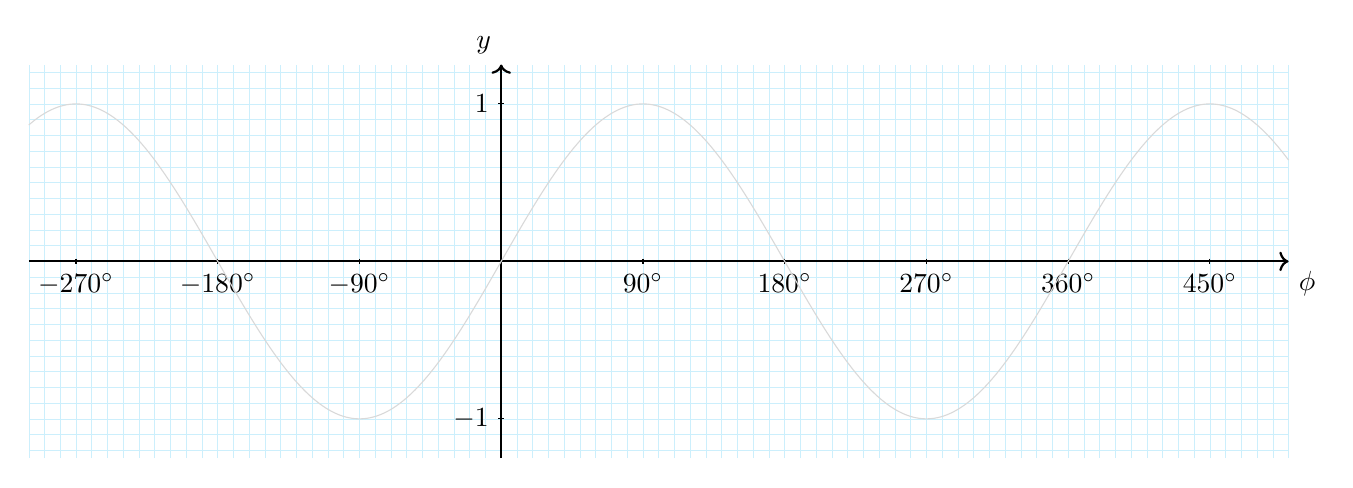
\begin{tikzpicture}
\draw[step = 0.2 cm, very thin, cyan!20] (-6, -2.5) grid ( 10, 2.5);
\draw[thick, ->] (-6,0) -- (10,0) node[anchor = north west] {$\phi$};
\draw[thick, ->] (0,-2.5) -- (0,2.5) node[anchor = south east] {$y$};

\foreach \x [evaluate=\x as \degree using int(\x*90)] in {-3,-2,-1,1,2,3,4,5}{ 
   \draw (\x *18mm, 1pt) -- (\x * 18mm, -1pt) node[anchor = north] {$\degree^\circ$};
   }
   
\foreach \y in {-1,1}
   \draw (1pt, \y *2cm) -- (-1pt, \y *2cm) node[anchor = east] {$\y$};

\draw[domain=-6:10,smooth,samples=200,variable=\x,gray!30] plot ({\x},{2*sin(\x*50)});
\end{tikzpicture}}%% END Definition

\newcommand{\trigsysDcos}{
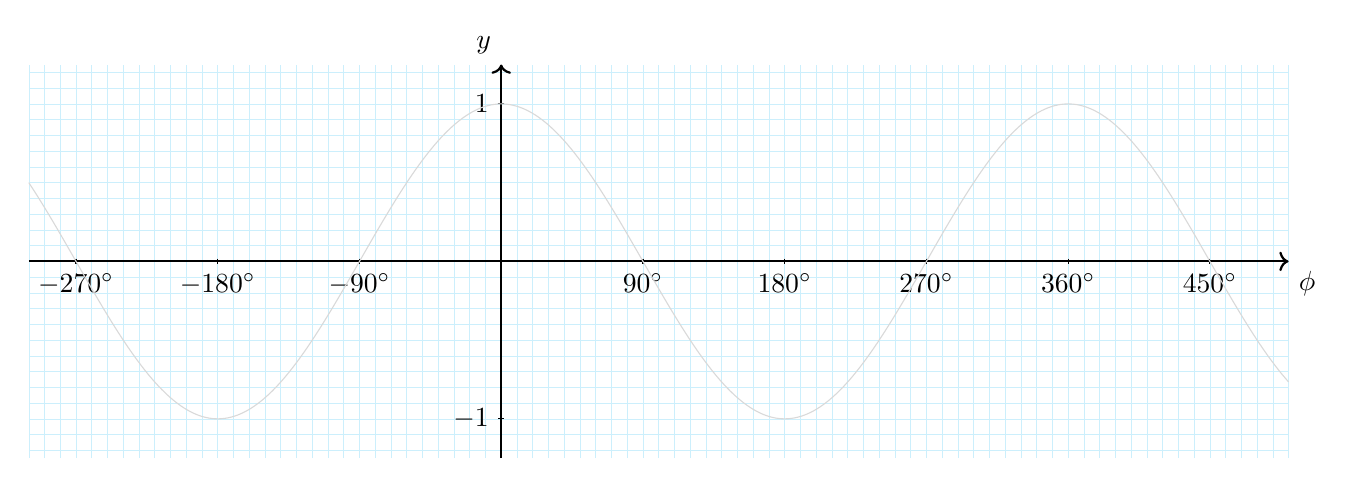
\begin{tikzpicture}
\draw[step = 0.2 cm, very thin, cyan!20] (-6, -2.5) grid ( 10, 2.5);
\draw[thick, ->] (-6,0) -- (10,0) node[anchor = north west] {$\phi$};
\draw[thick, ->] (0,-2.5) -- (0,2.5) node[anchor = south east] {$y$};

\foreach \x [evaluate=\x as \degree using int(\x*90)] in {-3,-2,-1,1,2,3,4,5}{ 
   \draw (\x *18mm, 1pt) -- (\x * 18mm, -1pt) node[anchor = north] {$\degree^\circ$};
   }
   
\foreach \y in {-1,1}
   \draw (1pt, \y *2cm) -- (-1pt, \y *2cm) node[anchor = east] {$\y$};

\draw[domain=-6:10,smooth,samples=200,variable=\x,gray!30] plot ({\x},{2*cos(\x*50)});
\end{tikzpicture}}%% END Definition



%% Aufgaben die entfernt werden, können durchaus im Kompendium
%% Qulltext bleiben.
\newcommand{\entfernteAufgabe}[3]{}
